\documentclass[12pt, letterpaper]{article}
\usepackage[utf8]{inputenc}
\usepackage{amsmath}
\usepackage{amssymb}
\usepackage{amsthm}
\usepackage[margin=1in]{geometry}
\usepackage{graphicx}
\usepackage[ruled,vlined]{algorithm2e}
\graphicspath{ {./img/} }


\author{Jeff Liu}
\title{Bayesian Modeling of Polar Sea Ice from IceSat-2 Freeboard Measurements}

\begin{document}

\maketitle

\section{Introduction}

Polar sea ice thickness is of interest to researchers for a variety of reasons including maritime navigation and climate change.
In 2018, NASA launched the IceSat-2 satellite, which relies a laser altimeter to help study polar sea ice.
To measure the thickness of this ice, the satellite takes measurements of ``freeboard'', which is the height of the ice above sea water.
Typically, 7/8 of the ice lies below water, so the freeboard can provide direct inference for the true thickness of the ice;
however, this measurement is complicated by an unknown amount of snow. Any snow present may weigh down the ice, pushing it deeper into the water,
which renders this 7/8 rule of thumb inaccurate.
\\\\
In response to this complication, scientists have devised a more sophisticated model that incorporates the amount of snow present into
the relationship between ice thickness and freeboard.
It relies on three additional parameters: the densities of the surrounding sea water, the sea ice in question, and the snow on top of the ice.
My goal in this paper is to incorporate this physical model as well as prior knowledge of the parameters to estimate the sea ice thickness
corresponding to a freeboard measurement of 0.1 meters. I will proceed to evaluate this estimate using Bayesian inference techniques
by defining a prior and likelihood and measuring the posterior.
\\\\
I will first proceed to elaborate on this physical model and formulate the Bayesian process to evaluate the expected ice thickness in section II,
including discussion of the assumptions, prior, hyper priors, forward model, likelihood functions, and posterior densities.
Following that, I will discuss the computational strategies for computing the posterior densities, including Markov Chain Monte Carlo,
in section III. Finally, I will report my model results and analyze model accuracy in section IV, and analyze and discuss the results in section V.

\newpage
\section{Formulation}

\subsection{Physical Model}
The physical model relating the ice thickness $H$, snow thickness $S$, and freeboard $H$ is the following:
\[
    F = \frac{\rho_w - \rho_i}{\rho_w} \left( H - S \frac{\rho_s}{\rho_w - \rho_i} \right),
\]
where $\rho_w$, $\rho_i$, and $\rho_s$ are the densities of the sea water, sea ice, and snow, respectively.
In the literature, it is given that Arctic seawater density $\rho_w$ ranges from 1010 to 1030 $kg/m^3$,
sea ice density $\rho_i$ ranges from 750 to 940 $kg/m^3$ while having an average value of 910 $kg / m^3$,
and snow density averages 300 $kg / m^3$ while ranging from 100 to 400 $kg / m^3$. In addition, I add a constraint
on sea ice thickness from Dr.\ Matthew Parno's Math 76 lecture on a similar model, where sea ice thickness ranges
from 0.1 to 5 meters while having an average value of 2 meters. No information is given on snow thickness, but it
is safe to say that snow thickness must be greater than or equal to zero meters.

\subsection{Assumptions}
To make this inference possible, I will have to make many assumptions because the given information is quite sparse.
\\\\
First, I must give some characterization to a prior density over these parameters. It is helpful that I have a given
range to work with for the parameters, but I will have to arbitrarily assume variances for all of them.
The potential bias introduced by of any poorly assumed variances is dampened by the fact that I have a predefined range of possibilities.
\\\\
In concert with these variance assumptions, I also assume that the prior densities are truncated Gaussian densities.
The reason for this choice is twofold. First, Gaussian densities are easily computed, and an added truncation is trivial
as long as we do not need to integrate to find the normalizing constant. Second, these truncations allow me to impose a strict
range upon the parameters, which helps with limiting the bias of arbitrarily chosen variances in my first assumption.
\\\\
My third assumption is that this model has additive noise. It is given that IceSat-2 can measure ice height within a few centimeters.
Since this measurement affects only the freeboard, which is not multiplied with anything in the physical model, I am assuming that this error
is additive. However, I will not make a hyperprior estimate on the exact amount of additive noise, and will reserve that to a hyperprior distribution
which I will discuss later.
\\\\
I will also need to make certain assumptions about the snow depth to make this model more easily computable. I visited a NASA website
discussing arctic snow depth over sea ice (https://earthobservatory.nasa.gov/images/146758/mapping-snow-on-arctic-sea-ice), and used the graphics
to semi-arbitrarily decide an average snow depth of 0.15 meters. However, giving an arbitrary estimate of the snow depth variance may
introduce too much bias into the model since I have no little information. Therefore, I will be modeling this variance as a hyperparameter
with a hyperprior as well.
\\\\
Because I am assuming truncated Gaussians for all prior densities, I will assume that the inverse-Gamma distribution will serve as a proper
hyperprior on my additive noise/error variance and my snow thickness variance. This is typically chosen for conjugacy reasons,
which I cannot take advantage of due to my truncations, but the general shape of the distribution is suitable for Gaussian variances anyway.
The ``hyper-hyper-priors'' $\alpha$ and  $\beta$ of the inverse-Gamma are chosen somewhat arbitrarily,
but this is not a huge issue since bias in hyper-hyper-parameters have little influence over the posterior. I will discuss my decision strategy
for these hyper-hyper-priors in a later subsection.
\\\\
My final assumption is that the prior parameters are independent. This is actually a poor assumption that I will revisit in the discussion section,
but I have no way to quantify the covariances of the parameters \emph{a priori}, so I have to make this assumption to make modeling possible.
Additionally, I make the assumption that the hyperparameters are independent from each other, and that the noise variance is also independent
from the parameters. This allows me to make some simplifications using conditional independence in my posterior formulation.

\subsection{Prior Formulation and Densities}
As I mentioned in the assumptions section, I chose the variances on the three densities rather arbitrarily.
I estimated the standard deviations of $\rho_w$ to 7, $\rho_i$ to 80, and $\rho_s$ to 90, and squared those to obtain the variances.
I also set the standard deviation of ice density to 2 meters, equal to the mean, to account for a fair amount of uncertainty, and squared that as well.
Finally, I guessed a mean standard deviation of snow density equal 0.2 meters, which is very wide. However, this value will not be going straight
into the prior model, since I will be modeling that standard deviation with an inverse-Gamma hyperprior. It remains useful for getting situated
and visualizing the prior, though.
\medskip
\begin{center}
\begin{tabular} { |c|c|c|c|c|c| }

\hline
parameter &  mean  & std.\ dev  & variance    & lower bound & upper bound \\
\hline
$\rho_w$  & 1020   &     7      &   49        &   1010      &    1030     \\
$\rho_i$  &  910   &    80      &   6400      &   750       &    940      \\
$\rho_s$  &  300   &    90      &   8100      &   100       &     400     \\
$H$       &  2.0   &    2.0     &   4.0       &   0.1       &    5.0      \\
$S$       &  0.15  &$\approx0.2$&$\approx0.04$&   0         &    unknown  \\
\hline

\end{tabular}
\end{center}
\medskip
Plots of the prior are shown on the next page. Note that the snow thickness plot is not a ``true'' prior; it is only an estimate
based on the hyperprior I will define next.

\begin{figure}[p]
\caption{Plots of Prior Densities}
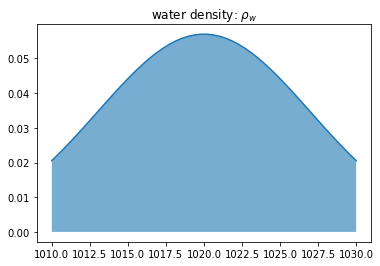
\includegraphics[width=0.5\textwidth]{prior_rw}
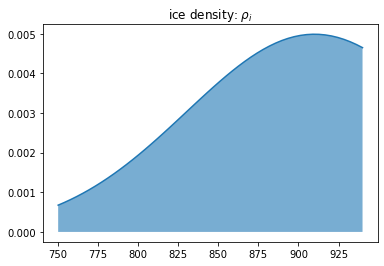
\includegraphics[width=0.5\textwidth]{prior_ri}
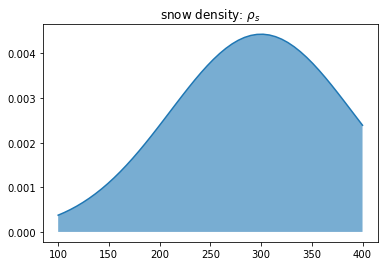
\includegraphics[width=0.5\textwidth]{prior_rs}
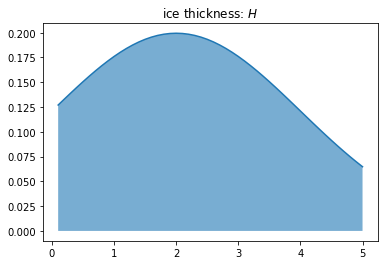
\includegraphics[width=0.5\textwidth]{prior_H}
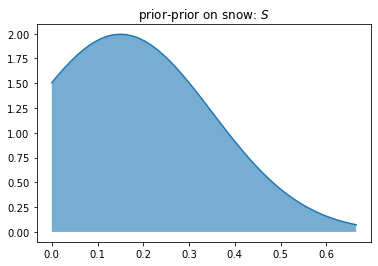
\includegraphics[width=0.5\textwidth]{prior_S}
\end{figure}

\newpage
\subsection{Hyperprior Formulation and Densities}
As mentioned in the assumptions, I chose to use inverse-Gamma densities as hyperpriors on the additive noise variance as well as the snow depth variance.
The Gamma distribution contains two parameters in the typical parametrization: $\alpha$ and $\beta$. These are largely arbitrary for my usage,
so I did a re-parametrization in terms of mean and variance, and used identities to convert them back to $\alpha$ and $\beta$ (from Wikipedia):
\[
    \mu = \frac{\beta}{\alpha - 1} \text{ for } \alpha > 1; \>
    \sigma^2 = \frac{\beta^2}{(\alpha-1)^2(\alpha-2)} \text{ for } \alpha > 2
\]
I chose hyperprior means equal to my estimates of the variances of the snow depth and error noise, which are the squared standard deviations.
For snow depth, I chose a semi-arbitrary estimate of 0.2 meters as mentioned earlier. For additive noise, I estimated three centimeters
based on the description of ``accurate to a few centimeters'' on IceSat-2. I chose the hyperprior variances assuming that the standard deviations
would be equal to the means. After that, I used the sympy package in Python to solve the equations for the hyper-hyper-parameters $\alpha$ and $\beta$.
Additionally, I also added a small ``nugget'' to each distribution to shift them a tiny bit away from zero to aid computation.
\medskip
\begin{center}
\begin{tabular} { |c|c|c|c|c|c|c| }

\hline
hyperparameter     &expected mean    &std.\ dev& variance &$\alpha$& $\beta$ & nugget \\
\hline
$\sigma^2_\epsilon$&$0.03^2=$ 9.0e-4 &  9e-4   &  8.1e-7  &  3.0   &  0.0018 & 0.0001 \\
$\sigma^2_S$       &$0.2^2=$ 0.04    &  0.04   &  1.6e-3  &  3.0   &   0.08  &  0.003 \\
\hline

\end{tabular}
\end{center}
\medskip

\begin{figure}[h]
\caption{Plots of Hyperprior Densities}
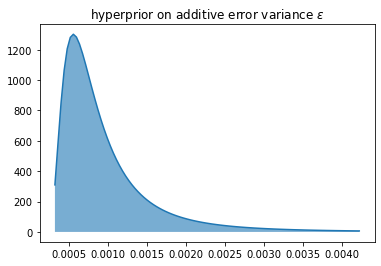
\includegraphics[width=0.5\textwidth]{hypprior_var_eps.png}
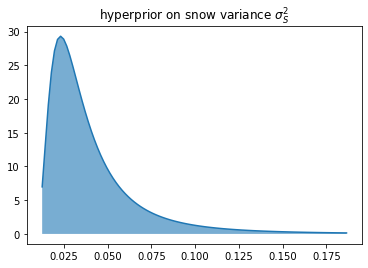
\includegraphics[width=0.5\textwidth]{hypprior_var_S.png}
\end{figure}

\newpage
\subsection{Forward Model and Likelihood Function}
Since I assume an additive Gaussian noise error, the likelihood function is a simple extension of the physical forward model.
Let $x$ be the five-dimensional vector containing the parameters $\rho_w$, $\rho_i$, $\rho_s$, $H$, and $S$,
and let $g(x)$ be the forward model predicting some freeboard value $F_{pred}$ from parameters $x$.
We can then describe the likelihood function as a Gaussian distribution with mean zero and variance $ \sigma^2_\epsilon$,
evaluated at the difference $F - g(x)$ as observed minus predicted.
\[
    f(F | x, \sigma^2_\epsilon) \sim N(0, \sigma^2_\epsilon)
\]
This is notably dependent on a variable noise variance, which I will explore in the next subsection on the hierarchical model.

\subsection{Hierarchical Model and Posterior Formulation}
Now I will proceed to discuss the posterior of the model, which contains hierarchical components regarding the noise and snow variances.
Traditionally, a non-hierarchical Bayesian model follows Bayes' rule, where the posterior is proportional to the prior times the likelihood:
\[
    f(x | F) \propto f(F | x) f(x)
\]
However, we have a hierarchical model which tries to incorporate the observation and obtain posterior hyperparameters as well.
These posterior hyperparameters show up here:
\[
    f(x, \sigma^2_\epsilon, \sigma^2_S | F) \propto f(F | x, \sigma^2_\epsilon) f(\sigma^2_\epsilon | \alpha_\epsilon, \beta_\epsilon)
    f(x | \sigma^2_S) f(\sigma^2_S | \alpha_S, \beta_S)
\]
I have dropped a few terms in this equation due to conditional independence. For example, $\sigma_S$ does not show up
in the likelihood function because F is conditionally independent of $\sigma_S$ given some value of x that has already been evaluated.
I also make use of my assumption that the two hyperparameter variances are independent as well, to make the joint distribution of
$\sigma^2_\epsilon$ and $\sigma^2_S$ just equal to the one we are interested in when the other is held constant.
Finally, I have left out the $\alpha$ and $\beta$ terms on the left side to save space; they are just constants here
and do not need to be listed, but I'm listing them to make clear which terms are inverse-Gamma hyperpriors.
\\\\
I will elaborate on the specific computation of this posterior, as well as the hierarchical separation of the parameters and hyperparameters,
in the next section.

\subsection{Expected Value of Ice Thickness}
The solution to my answer is relatively simple after computing the posterior density. Since I am purely making an inference on the parameters,
I can just compute $\mathbb{E}[x_{post}]$ and then extract the specific expected value and posterior density on ice thickness $H$.

\newpage
\section{Solution and Computation Strategy}

\subsection{Non-Conjugacy and Markov Chain Monte Carlo}
My model is non-conjugate in two areas. First, the physical model is simple but non-linear, so no linear algebra identities can be used to
analytically derive the distributions. Second, I chose to use truncated Gaussians, which have complex normalizing constants that render conjugacy impossible
in and of itself. These conditions leave sampling as the best technique to derive the posterior, as we can take advantage of the Central Limit
Theorem to prevent the exponential growth in computational complexity for numerical integration of a multi-dimensional density.
\\\\
Within sampling techniques, I chose to use Markov Chain Monte Carlo due to the difficulty of generating direct samples from the truncated prior density.

\subsection{Hierarchical MCMC and Gibbs Sampling}
With a hierarchical model, it is easier to break up each sampling step into three distinct steps: one for the parameters $x$
and one for each hyperparameter $\sigma^2_\epsilon$ and $\sigma^2_S$. This technique, called Gibbs sampling, is computationally easier
to evaluate. In each sub-step, I can hold the other variables constant, reducing the amount of required computation. In addition,
I free up the hyperparameters to be sampled independently of the parameters. Gibbs sampling will necessitate a modification to 
the formulation where each parameter and hyperparameter is isolated in the posterior.
\\\\
For the sub-step involving the parameters $x$ while the hyperparameters are held constant, the marginal posterior on $x$ looks like this,
which can then be simplified by dropping $\sigma^2_S$ in the likelihood function and $\sigma^2_\epsilon$ in the prior
due to our independence and conditional independence assumptions on the parameters.
\begin{eqnarray*}
    f(x | F, \sigma^2_\epsilon, \sigma^2_S) & \propto & f(F | x, \sigma^2_\epsilon, \sigma^2_S) f(x | \sigma^2_\epsilon, \sigma^2_S) \\
                                            & \propto & f(F | x, \sigma^2_\epsilon) f(x | \sigma^2_S)
\end{eqnarray*}
For the sub-step involving $\sigma^2_\epsilon$ while $x$ and $\sigma^2_S$ are held constant, the marginal posterior looks like this,
which can be simplified by dropping dependence on $\sigma^2_S$ entirely (since I assume the two hyperpriors are independent),
and dropping both dependencies on $x$ and $\sigma^2_S$ in the hyperprior (again due to the same assumption).
\begin{eqnarray*}
    f(\sigma^2_\epsilon | F, \sigma^2_S) & \propto & f(F | x, \sigma^2_\epsilon, \sigma^2_S) f(\sigma^2_\epsilon | x, \sigma^2_S) \\
    f(\sigma^2_\epsilon | F)             & \propto & f(F | x, \sigma^2_\epsilon) f(\sigma^2_\epsilon)
\end{eqnarray*}
Finally, for the sub-step involving $\sigma^2_S$ while $x$ and $\sigma^2_\epsilon$ are held constant, the marginal posterior
looks like this: 
\begin{eqnarray*}
    f(\sigma^2_\S | F, \sigma^2_\epsilon) & \propto & f(F | x, \sigma^2_\epsilon, \sigma^2_S) f(\sigma^2_S | x, \sigma^2_\epsilon) \\
                                          & \propto & f(F | x, \sigma^2_\epsilon) f(x | \sigma^2_S) f(\sigma^2_S)
\end{eqnarray*}
In the $\sigma^2_S$ step, I first simplify by dropping $\sigma^2_S$ in the likelihood due to conditional independence given fixed $x$.
Next, I must expand the hyperprior, since I do not have a calculation for the density on $\sigma^2_S$ given $x$.
I do this expansion using Bayes' rule to ``flip'' the density into something I can calculate, which is just a prior and hyperprior.

\subsection{Metropolis-Within-Gibbs and Proposal Distribution}
Using these new posterior distributions, I executed my Gibbs sampling using the Metropolis-Hastings rule for each sub-step.
Together with Gibbs sampling, this creates three ``orthogonal'' walking steps per iteration, and the overall combination of these
techniques is called Metropolis-Within-Gibbs sampling.
\\\\
For the Metropolis-Hastings rule, I chose to use either univariate or multivariate Gaussians for all proposal densities.
This is convenient because it removes the need to consider the proposal ratios when calculating the acceptance ratio,
since Gaussians are symmetric. I scaled the proposal standard deviations of the parameters together,
such that they were equally proportional to their respective prior standard deviations. I chose that scaling factor
rather arbitrarily though trial-and-error in an attempt to make the autocorrelation as low as possible.
The proposal standard deviations of my hyperparameters were each chosen independently as well.
The standard deviations are listed below:
\medskip
\begin{center}
\begin{tabular} { |c|c|c|c|c|c|c| }

\hline
$\rho_w$ & $\rho_i $& $\rho_s$ & $H$ & $S$ & $\sigma^2_\epsilon$ & $\sigma^2_S$ \\
\hline
1.96     & 22.4     & 25.2     &0.56 &0.056&    1.05e-3          & 0.05         \\
\hline

\end{tabular}
\end{center}
\medskip
Note that since my Metropolis-Hastings step with regard to the first five parameters is contained with one vector $x$,
the five standard deviations make up a covariance matrix where there is an independence assumption on the components
(which was what I assumed). As I have stated in the assumptions section, I will revisit the impact of this in the discussion section.


\subsection{Overview of Software Tools}
To do this computation, I have used the Jupyter Notebook interface with classic Python scientific computing and statistics packages
such as Matplotlib, Numpy, Scipy, and Sympy. I additionally import a specific function from Pandas for a more sophisticated plot,
although I do not use Pandas for any data manipulation.
\\\\
I wrote most of the code myself, with small parts taken from Dr.\ Parno's example code in places such as plotting, MCMC setup,
and autocorrelation analysis.

\newpage
\subsection{Pseudocode}
Here, I will outline the general algorithmic process I take to compute the Markov Chain Monte Carlo.
Notably, I will use logarithms of all calculated densities to increase computational performance.
Additionally, I chose to record 10,000 iterations, since my autocorrelation was rather high.

\medskip
\begin{algorithm}[H]
\SetAlgoLined
\KwResult{Samples from the posterior distributions of the parameters and hyperparameters}
 
Define constants\\
Set up functions to evaluate the log-prior\\
Set up functions to evaluate the log-hyperpriors\\
Set up functions to evaluate the log-likelihood function\\
Create initial conditions for MCMC and prepare proposal distribution\\

\For{range from 1 to 10000}{
    propose new point for $x$ and compute the acceptance ratio $\gamma$\\
    \eIf{random number 0 to 1 $< \gamma$}{
        set next $x$ to proposed $x$\\
    }{
        set next $x$ to previous $x$\\
    }
    propose new point for $\sigma^2_\epsilon$ and compute the acceptance ratio $\gamma$\\\\
    \eIf{random number 0 to 1 $< \gamma$}{
        set next $\sigma^2_\epsilon$ to proposed $\sigma^2_\epsilon$\\
    }{
        set next $\sigma^2_\epsilon$ to previous $\sigma^2_\epsilon$\\
    }
    propose new point for $\sigma^2_S$ and compute the acceptance ratio $\gamma$\\\\
    \eIf{random number 0 to 1 $< \gamma$}{
        set next $\sigma^2_S$ to proposed $\sigma^2_S$\\
    }{
        set next $\sigma^2_S$ to previous $\sigma^2_S$\\
    }
}

Record, plot, and analyze results\\
Compute Integrated Autocorrelation time and standard error\\
Check Posterior Predictive\\
\caption{Metropolis-Within-Gibbs MCMC}
\end{algorithm}

\newpage
\section{Results}

\subsection{Sampling Results and Posterior Densities}
After 10,000 iterations, I recorded the following posterior plots:
\begin{figure}[h]
\caption{Scatter Matrix of Posterior on $x$}
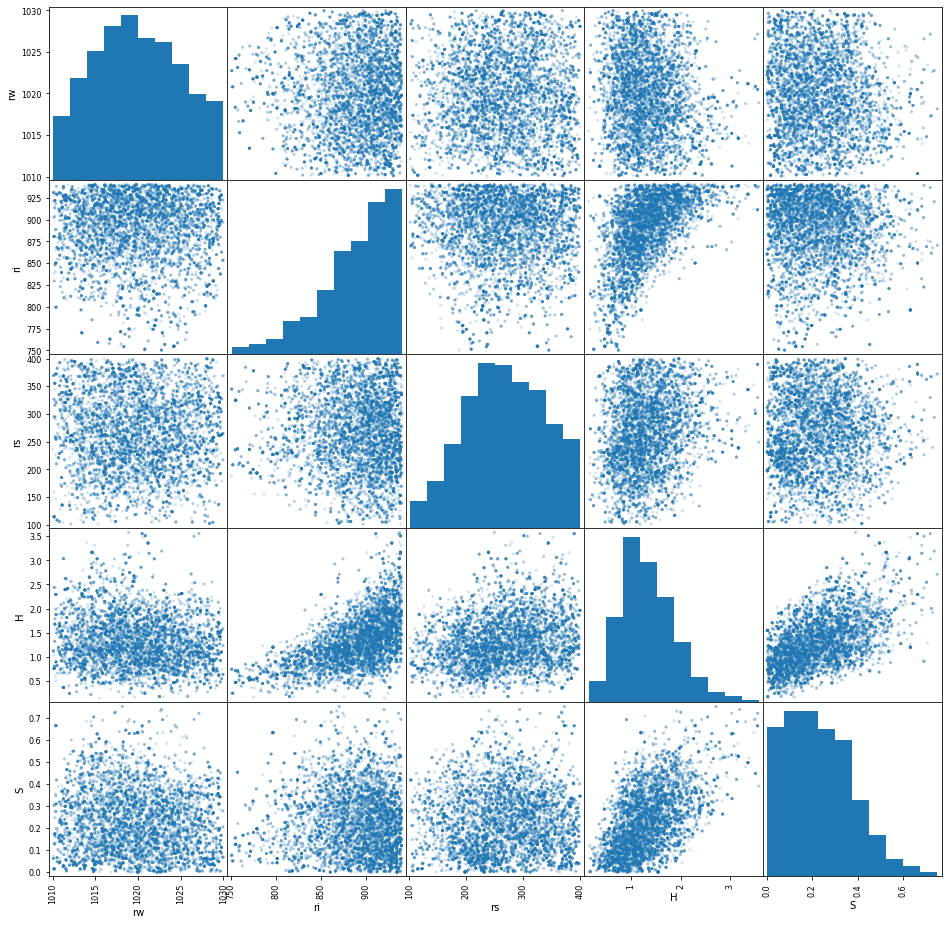
\includegraphics[width=\textwidth]{posterior_matrix.png}
\end{figure}
\begin{figure}[h]
\caption{Posterior Histograms on Hyperparameters and Ice Thickness}
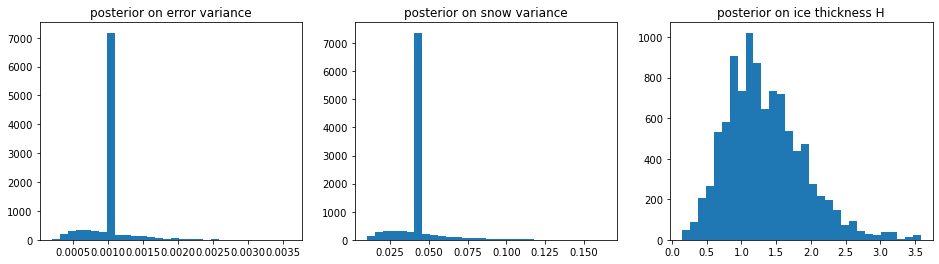
\includegraphics[width=\textwidth]{posteriors.png}
\end{figure}

Out of the five primary parameters, most of the densities remained similar to the priors. However, the snow density $\rho_s$ was shifted down slightly,
and the variance of the ice thickness $H$ was significantly tightened. Furthermore, observing the scatter matrix, significant covariances were
found in the posterior. This makes sense; our physical model contains many ratios, which means that the freeboard will stay constant when
certain parameters move in tandem.
\\\\
The posteriors on the error and snow variances are have become extremely tight, as seen in the histograms. The ice thickness
posterior has grown reasonably tight too. Whereas the prior had a mean and standard deviations of 2.0 meters each, the posterior
has a mean of 1.34 meters and standard deviation of only 0.55 meters. This is still a pretty wide curve, but is an insightful result
compared to the absolute uncertainty of the prior.

\subsection{Central Limit Theorem, Autocorrelation, and Error Analysis}
Since I am dealing with samples, the Central Limit Theorem applies to the model accuracy. Because I am working with Markov Chain Monte Carlo,
each sample is not independent, so the strict CLT does not apply. To use the CLT, I performed autocorrelation analysis to quantify
the lack of independence between samples.
\begin{figure}[h]
\centering
\caption{Autocorrelation Functions of Posterior w.r.t. Lag}
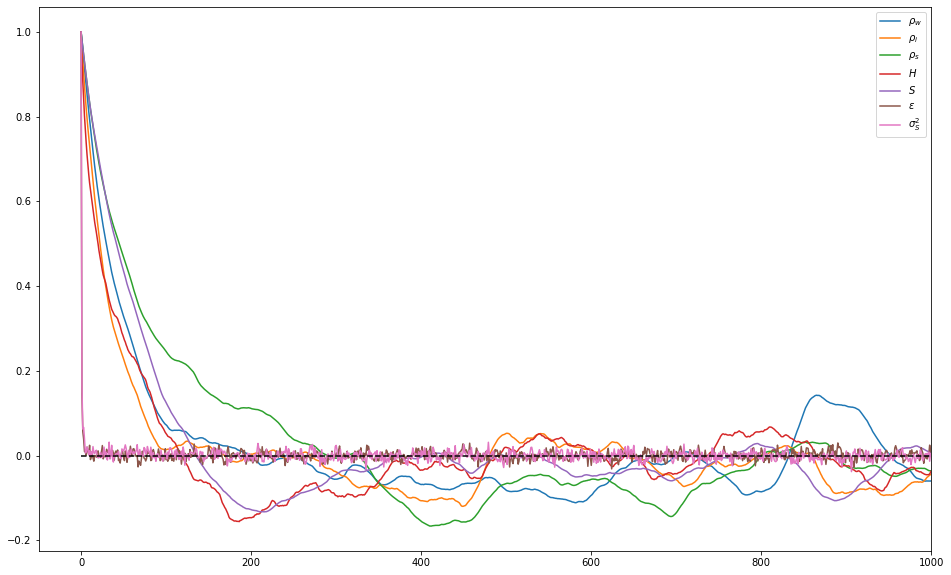
\includegraphics[width=0.85\textwidth]{autocorr.png}
\end{figure}
\\\\
The autocorrelation functions for the hyperpriors $\sigma^2_S$ and $\sigma^2_\epsilon$ look excellent, quickly decaying to zero,
but the five parameters in $x$ are a bit lackluster. They take a long time to decay, and even have a low negative autocorrelation
for large parts of the chain.
\\\\
By integrating the autocorrelation functions, we obtain the integrated autocorrelation time (IACT). This value serves as a coefficient
in the modified CLT for MCMC. The IACTs for all seven parameters/hyperparameters are below:
\medskip
\begin{center}
\begin{tabular} { |c|c|c|c|c|c|c| }

\hline
$\rho_w$ & $\rho_i $& $\rho_s$ & $H$ & $S$ & $\sigma^2_\epsilon$ & $\sigma^2_S$ \\
\hline
37.81    &  12.36   &  58.08   &15.86&35.04&     1.93            & 1.41         \\
\hline

\end{tabular}
\end{center}
\medskip
As expected, the IACT indicates fast convergence for the hyperparameters, while the parameters lag behind. This will negatively impact the
standard error. In addition, something to note is that I did not account for modeling error from negative autocorrelation. The standard
error should perhaps be even higher to account for this, which is a potential limitation of my model. The full summary statistics of the posterior,
along with calculated standard error, are below:

\medskip
\begin{center}
\begin{tabular} { |c|c|c|c|c|c|c|c| }

\hline
             &$\rho_w$ & $\rho_i $& $\rho_s$ & $H$ & $S$ & $\sigma^2_\epsilon$ & $\sigma^2_S$ \\
\hline
mean         & 1019.91  &887.81    & 267.57  & 1.34& 0.23&    0.001            &  0.043       \\
std.\ dev    & 4.99     & 40.25    & 69.47   &0.55 & 0.15&    0.003          &   0.0123        \\
std.\ error  & 0.31     & 1.42     & 5.29     &0.02 &0.01&    4.0e-6         &  1.46e-4         \\
\hline

\end{tabular}
\end{center}
\medskip

\subsection{Posterior Predictive}
As a final check on my model, I used the samples of the Markov Chain Monte Carlo to also sample a posterior predictive on freeboard.
I did this by stepping through the iterations and computing the forward model plus a noise value with the current $\sigma^2_\epsilon$.
\begin{figure}[h]
\centering
\caption{Posterior Predictive}
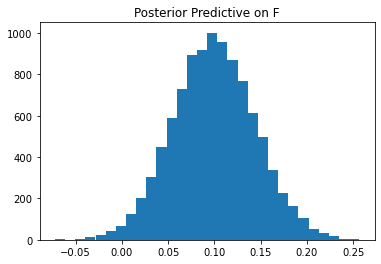
\includegraphics[width=0.4\textwidth]{predictive.png}
\end{figure}
\\\\
The posterior predictive is understandably very wide to account for a lot of uncertainty, but our measured value of 0.1 is in the middle,
so this looks qualitatively reasonable.

\section{Discussion}

\subsection{Sea Ice Thickness}
The original goal of this analysis was to find a posterior on the sea ice thickness, and I have found one. My model estimates that
the expected value of the ice thickness causing the 0.1 meter freeboard measurement is 1.34 meters thick. As stated earlier,
my model puts a wide range of possibilities with the 0.55 meter standard deviation, but we nonetheless have a reasonable expectation now.
Additionally, there is a low standard error of 0.02 meters on this expected value, so we can be reasonably sure that our expectation
is accurate. With further measurements, this posterior can be further shrunk to more precisely show a range of thickness values.

\subsection{Observations on Posterior}
The posterior revealed a lot about the internal structure of the model despite only having a single freeboard measurement to work off of.
For example, it clearly learned the nature of the covariances between the parameters without any additional input. Looking at the
scatter matrix, we can see that ice density and ice thickness have a strong positive covariance, and ice thickness with snow thickness as well.
These both reflect intuitive ideas about the physics of sea ice. The denser the ice is, the thicker it will need to be to have enough buoyancy
to stay floating at the same freeboard. Similarly, the more snow there is, the more ice will be needed to counterbalance the snow mass with
buoyancy as well. There are likely more nuances in the model that depend on three or more variables acting in tandem, but upon
initial assumption, this insight is fascinating yet extremely intuitive.
\\\\
Some additional observations can be gleaned as well. The model predicts a higher ice density than we originally set in the prior,
and a lower snow density, although the snow variance is very wide. Furthermore, it predicts a noise standard deviation of only one centimeter,
which puts pretty high confidence on IceSat-2's precision.

\subsection{Revisiting Assumptions and Potential Bias}
The model contains a lot of insight, but relies on several assumptions, some of which may be problematic. First of all,
the model seems to not have affected the water and snow densities much. Selecting a different prior may have made a large difference
as a result. In general, this model relies heavily on preexisting knowledge because of the tiny amount of data present.
\\\\
Another potential source of bias is the independence assumption between the model parameters, and consequently the choice
of a diagonal covariance matrix for the proposal distribution. As we can see in the posterior scatter matrix, there is clearly
strong covariance in the model, which does not agree with our prior. I suspect that this strong covariance has to do with the difficulty I
experienced in getting the autocorrelation functions of my Markov Chains to decay, and it may also be the reason behind the negative covariance.
When a zero-covariance model is proposed, the acceptance rate will be artificially deflated, since many of the proposal steps will go in the
``wrong'' direction to the model covariance. This results in an unusually small step size, which can increase autocorrelation. Furthermore,
The high-covariance nature of the model may lend itself to a ``yo-yo'' like back-and-forth on accepted proposal steps, which can cause negative
autocorrelation. This negative autocorrelation may be artificially deflating the standard errors of my parameters. However, I still have a large sample size,
so the convergence of the model should still be sufficient compared to how much uncertainty is already present.

\subsection{Conclusion}
In conclusion, the model has its issues, but the general uncertainty of the model combined with the large sample size allow its inferences to be valid.
We can be reasonably sure that the model's wide range of predictions is true to life, as long as our prior distributions are accurate as well.
With further data, we can hopefully bring our 1.34 meter estimation of the sea ice thickness closer to the true value.

\end{document}
